\renewcommand{\chaptername}{Chapter} 
\chapter{Reanalysis of psychophysical biomarkers}\label{chap8}
The main objective of GLM-HMM modelization was to apply a probabilistic model to detect hidden states in participants' responses. The GLM-HMM model provided a structured approach for estimating posterior state probabilities on a trial-by-trial basis and constructing a transition matrix, which allowed us to analyze the likelihood of participants remaining in or transitioning between states. Unlike traditional signal detection theory tasks, where a ground truth exists and ROC curves can be used to assess performance, our challenge was the absence of a correct response in the reverse correlation experiment. This made it impossible to directly determine how many states participants could switch between. To overcome this, we conducted extensive simulations with known true states, enabling us to optimize model fitting using maximum a posteriori (MAP) estimation by selecting the most appropriate priors.\newline
Applying these optimized priors led to several unexpected findings. Most notably, patients showed a stronger tendency to remain in the perseverative state, making significantly fewer transitions back to an engaged, stimulus-driven decision mode. This suggests that once patients enter a perseverative state, they struggle to re-engage with external sensory information, whereas controls demonstrate greater flexibility, dynamically adjusting their responses based on stimulus input.\newline
One of the key findings in Chapter 4 was that internal noise, rather than just internal representation, plays a major role in differentiating patients from controls. However, we recognized that internal noise estimates from the double-pass method were contaminated by perseveration in patients, leading to inflated values. Thus, a primary goal in this chapter was to assess whether removing perseverative trials would reduce internal noise estimates. Our results confirmed this hypothesis: after filtering out perseverative trials, internal noise values—previously estimated through the confidence interval of the GLM—decreased significantly, supporting the idea that perseveration artificially inflates internal noise measurements in patients.\newline
These findings highlight the importance of distinguishing true internal noise from noise introduced by behavioral biases, reinforcing the need for probabilistic models like GLM-HMM to uncover underlying cognitive states rather than relying solely on traditional psychophysical measures.

\section{Qualitative impact of new methodologies on Kernel typicality}

In Chapter \ref{chap3}, we introduced the linear models used to estimate kernels (internal representations through weighted sums and GLMs) in reverse correlation tasks. These models have been applied to various experimental paradigms. Later, in Chapter \ref{chap5}, we discussed the limiting factors affecting their performance.

Our primary objective was to detect perseverative trials and obtain a more accurate estimation of the GLM kernel for engaged trials. However, as discussed in the previous chapter, simply removing perseverative trials does not necessarily improve the similarity of kernel typicality between perseverative patients and controls, figure \ref{fig:kernels_segments_methods} and \ref{fig:kernel_comparison_methods} showing that after removing perseverative trials, the estimated kernel magnitudes tend to be lower. One possible explanation is that a significant proportion of patient responses occur in the perseverative state. Specifically, while controls have an average of 119 engaged trials out of 150 (80\%), patients have significantly fewer, with only 62 engaged trials out of 150 (41\%).

This substantial reduction in trial count affects kernel estimation, as a reliable estimation requires at least 200 trials (as demonstrated in Figure \ref{fig:experiment}). Consequently, the loss of trials in perseverative patients limits our ability to obtain robust kernel estimates, highlighting the challenge of accurately characterizing their internal representations, as already been shown by the simulation validation in chapter \ref{chap7}.


\begin{figure}[H]
    \centering
    \includegraphics[width=17cm,height=7cm]{MainLayout/Images/chapter8/kernels_segments_methods.jpg}
    \caption{Main Title for First Image \\ \small Subtitle for the first graphic.}
    \label{fig:kernels_segments_methods}
\end{figure}

In figure \ref{fig:kernel_comparison_methods}, we present a scatter plot comparing patients' kernel typicality in dark blue—how closely their kernel resembles that of a control group in orange—across three different methods: kernel-CI (Classification Images or weighted sum) for all trials, kernel-GLM (Generalized Linear Model) for all trials, and kernel-HMM, which represents the GLM kernel computed only for engaged trials.
The size of each point represents the number of engaged trials for each participant, with data categorized into two groups: controls (n = 114) and patients (n = 70). Participants were further classified based on a cut-off value for engaged trials: those with fewer engaged trials are considered "less engaged," while those exceeding the cut-off are classified as "highly engaged."
Our findings indicate that patients with fewer engaged trials tend to deviate further from the diagonal line, which represents the similarity between methods. This effect is particularly evident in the third plot, where patients with fewer engaged trials show a pronounced divergence from the diagonal, highlighting the impact of engagement level on kernel similarity across methods.

\begin{figure}[H]
    \centering
    
\includegraphics[width=17cm,height=7cm]{MainLayout/Images/chapter8/kernel_comparison_methods.jpg}
    \caption{Main Title for First Image \\ \small Subtitle for the first graphic.}
    \label{fig:kernel_comparison_methods}
\end{figure}
In Figure \ref{fig:kernel_comparison_types_methods}, we present patients classified based on their pathological score in the MEC (Montreal Evaluation of Communication) assessment, which is discussed in detail in Chapter \ref{chap2}. The MEC remains one of the most widely used communication batteries by speech pathologists. As shown in the scatter plot, we defined patients according to a cut-off score of 9, with those scoring above this threshold (MEC > 9) represented in dark blue, indicating no pathological impairment, while those scoring 9 or below (MEC<= 9) are shown in light blue, indicating a prosody perception deficit.

Similar to Figure \ref{fig:kernel_comparison_methods}, the size of the points in the plot represents the number of engaged trials per patient. On average, patients with MEC > 9 had 71 engaged trials, whereas patients with MEC<= 9 had an average of 69 engaged trials.
Regarding kernel typicality across methods, control participants showed consistently high values across all approaches, with kernel-CI at 0.92, kernel-GLM at 0.93, and kernel-HMM at 0.91. Among patients with MEC<= 9, kernel typicality was lower, with values of 0.61 for kernel-CI, 0.57 for kernel-GLM, and 0.57 for kernel-HMM. Patients with MEC > 9 exhibited intermediate kernel similarity, with scores of 0.74 for kernel-CI, 0.75 for kernel-GLM, and 0.68 for kernel-HMM. These findings suggest that kernel similarity decreases in patients with greater prosody perception deficits, particularly when estimated using the GLM or HMM methods.
\begin{figure}[H]
    \centering
    
\includegraphics[width=17cm,height=7cm]{MainLayout/Images/chapter8/kernel_comparison_types_methods.jpg}
    \caption{Main Title for First Image \\ \small Subtitle for the first graphic.}
    \label{fig:kernel_comparison_methods}
\end{figure}

The Mann-Whitney U tests further confirm these differences, figure \ref{fig:kernels_segments_types} showing significant distinctions between patients and controls but weaker effects when comparing MEC<= 9 and MEC > 9 patients.
Comparing MEC<= 9 vs. MEC > 9 patients, there is no significant difference in kernel similarity across all methods (p > 0.05). This suggests that prosody deficits do not strongly impact kernel similarity within the patient group.
Comparing MEC<= 9 patients to controls, we find highly significant differences across all kernel estimation methods (p = 0.000), with patients showing significantly lower kernel similarity. This indicates that patients with severe prosody perception deficits exhibit markedly different kernel structures compared to controls.
Comparing MEC > 9 patients to controls, there are significant but less pronounced differences (p = 0.002 - 0.004), indicating that patients with mild or no prosody deficits still show reduced kernel similarity compared to controls, but to a lesser extent than MEC<= 9 patients. 
Which concludes there is no differences in these three methodes at level of kernel similarity.
\begin{figure}[H]
    \centering
    \includegraphics[width=17cm,height=7cm]{MainLayout/Images/chapter8/kernels_segments_types.jpg}
    \caption{Main Title for First Image \\ \small Subtitle for the first graphic.}
    \label{fig:kernels_segments_types}
\end{figure}

\section{Qualitative impact of new methodologies on Internal noise}
By examining the scatter plots comparing internal noise across different estimation methods, we observe distinct patterns between patients and controls. The Double-Pass (DP) method, which does not account for trial-by-trial state transitions, tends to overestimate internal noise in patients with low engagement, as seen in the upper-left quadrant of the DP vs. GLM-HMM plot. This suggests that many of these patients had perseverative trials that artificially inflated their noise estimates. In contrast, when using the GLM-HMM method, which isolates engaged trials, internal noise estimates decrease, particularly for low-engagement patients. Highly engaged patients, represented by larger points, exhibit more stable noise estimates across all methods, indicating that their decision-making is less affected by perseveration.

The GLM method, which estimates noise across all trials without distinguishing between states, generally reports higher internal noise than GLM-HMM, particularly in patients with low engagement. This highlights the importance of accounting for perseverative trials in noise estimation, as their inclusion in GLM leads to inflated confidence intervals and higher uncertainty. Controls, on the other hand, consistently show low internal noise across all methods, aligning closely with the diagonal in all plots. The absence of points in the lower-right quadrant of the DP vs. GLM-HMM plot confirms that patients with low DP noise also have low noise when assessed through engaged trials, reinforcing the idea that noise, when present, is pervasive rather than trial-specific.

Overall, these findings demonstrate that perseveration significantly impacts internal noise estimation in patients, leading to overestimation in DP and GLM methods. The GLM-HMM approach provides a more refined measure by focusing only on engaged trials, revealing that some patients had artificially high noise estimates due to perseverative responses. This highlights the necessity of distinguishing between engaged and perseverative trials when assessing perceptual stability in patient populations.
\begin{figure}[H]
    \centering
    
\includegraphics[width=17cm,height=8cm]{MainLayout/Images/chapter8/internal_noise_comparison_glms.jpg}
    \caption{Main Title for First Image \\ \small Subtitle for the first graphic.}
    \label{fig:internal_noise_comparison_glms}
\end{figure}
The internal noise estimates across different methods reveal key distinctions between control participants and patients, particularly those with prosody perception deficits (MEC<= 9). In the Double-Pass (DP) method, there is a significant difference between patients with MEC<= 9 and controls (p = 0.004), with patients exhibiting much higher noise levels (2.89 vs. 0.89). However, no significant difference is found between MEC<= 9 and MEC > 9 patients (p = 0.409), suggesting that DP does not capture within-patient variability effectively.

This difference persists in the GLM-based estimation, but with even greater separation, as noise in the MEC<= 9 group rises to 8.33, compared to 4.4 in MEC > 9 patients and 1.63 in controls. The GLM method shows a highly significant difference between MEC<= 9 and controls (p = 0.000), as well as between MEC > 9 and controls (p = 0.027), indicating that patients, regardless of severity, exhibit higher noise levels than controls. However, no significant difference is found between MEC<= 9 and MEC > 9 patients (p = 0.138), reinforcing that GLM captures overall group-level differences but not fine-grained variations within patients. The fact that GLM estimates higher noise suggests that perseveration inflates confidence intervals when all trials are considered.

When using the GLM-HMM method, which isolates engaged trials, internal noise in MEC<= 9 patients is significantly reduced to 3.88, revealing a more accurate measure of perceptual variability. Unlike DP and GLM, GLM-HMM not only maintains a significant difference between MEC<= 9 and controls (p = 0.001) but also between MEC<= 9 and MEC > 9 patients (p = 0.030). This suggests that perseveration in MEC > 9 patients was more prevalent in repeated trials, leading to inflated noise estimates in DP and GLM. However, no significant difference is found between MEC > 9 and controls in GLM-HMM (p = 0.133), indicating that after removing perseverative trials, the noise levels of MEC > 9 patients resemble those of controls.
\begin{figure}[H]
    \centering
    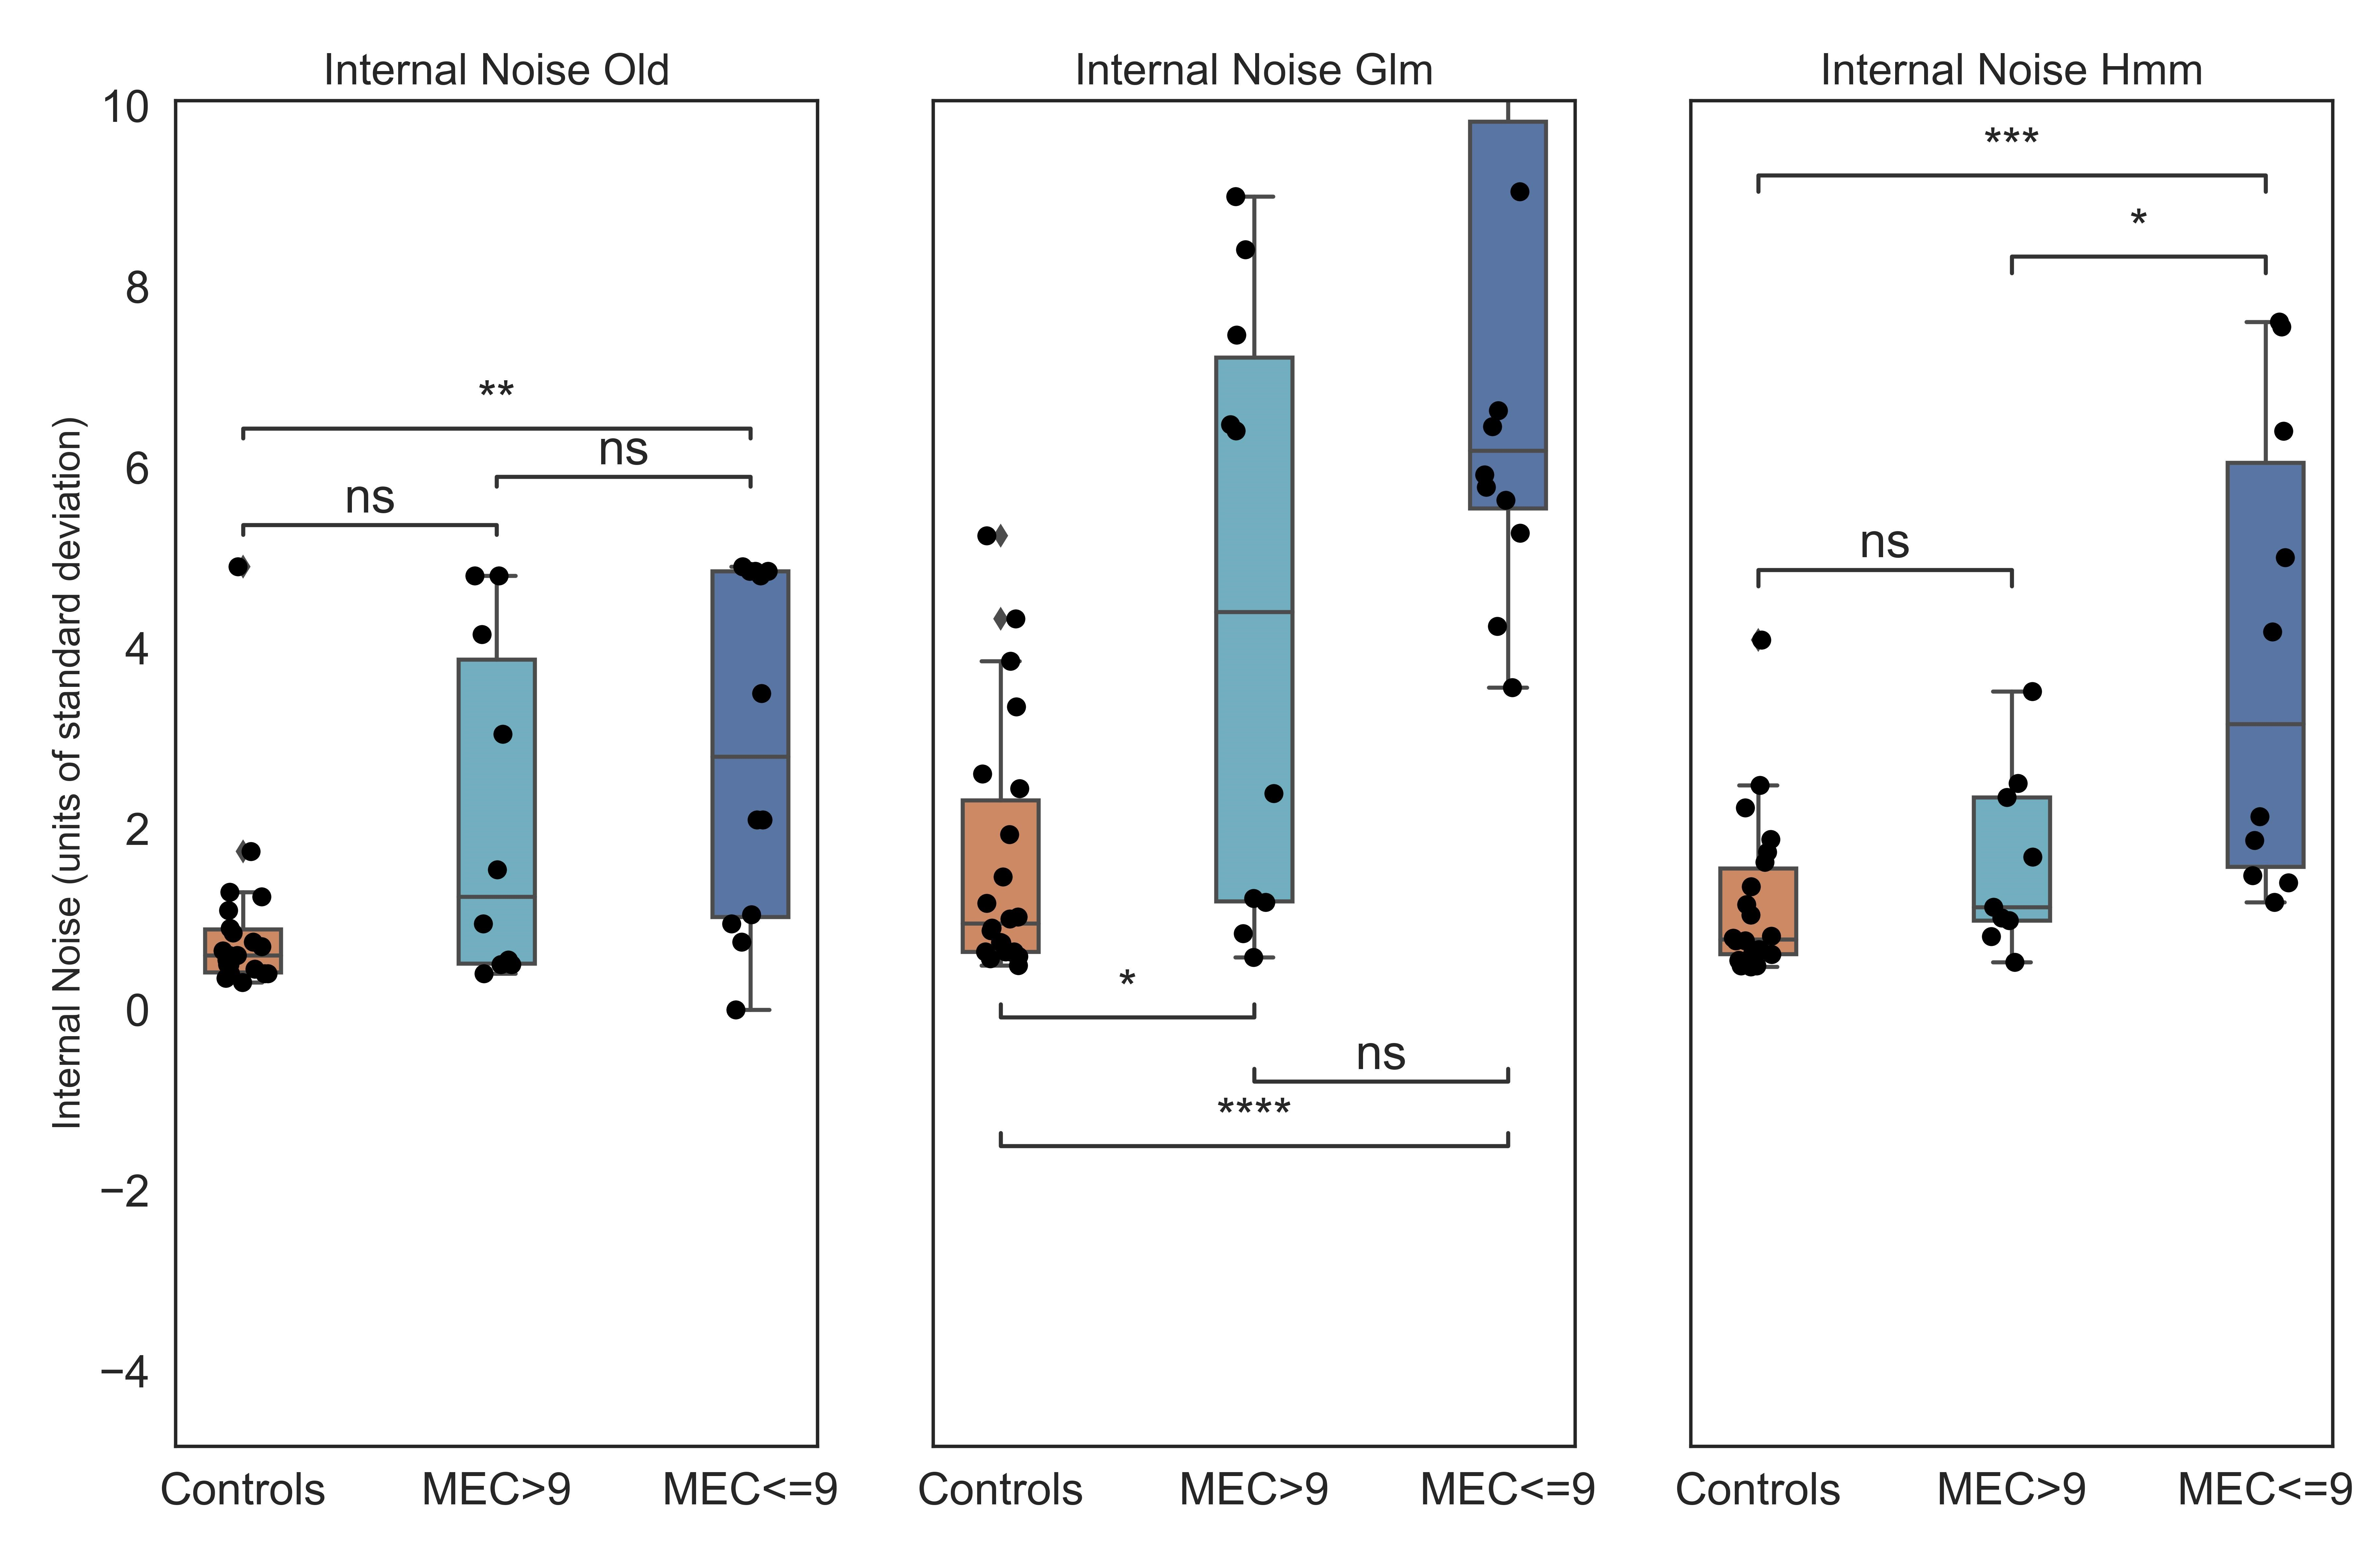
\includegraphics[width=17cm,height=10cm]{MainLayout/Images/chapter8/internal_noise_types_glms.jpg}
    \caption{Main Title for First Image \\ \small Subtitle for the first graphic.}
    \label{fig:internal_noise_comparison_types_glms}
\end{figure}
In the third plot of figure \ref{fig:internal_noise_comparison_glms} (Internal Noise HMM vs. DP), a key trend emerges: DP systematically overestimates internal noise compared to GLM-HMM, especially in patients. Many of these patients cluster in the upper-left quadrant, indicating that their DP-based noise estimates were inflated by perseverative trials. The GLM-HMM method, which isolates engaged trials, provides significantly lower estimates, suggesting that perseveration was artificially increasing noise in DP trials. In contrast, controls (orange points) and high-engagement patients (larger points) align more closely with the diagonal, indicating that their noise estimates remain more stable across methods.
\begin{figure}[H]
    \centering
    
\includegraphics[width=17cm,height=7cm]{MainLayout/Images/chapter8/internal_noise_comparison_types_glms.jpg}
    \caption{Main Title for First Image \\ \small Subtitle for the first graphic.}
    \label{fig:internal_noise_comparison_types_glms}
\end{figure}
\section{Probability of transition to perseveration as a new biomarker} 
The probability of transitioning between states is a key variable extracted from the GLM-HMM model. A critical question was whether these transition probabilities differ across groups, providing insight into behavioral flexibility. Our analysis revealed the following patterns:

Comparing MEC<= 9 and MEC > 9 patients, no significant difference was found in the probability of transitioning to a perseverative state (p = 0.079) or to a non-perseverative state (p = 0.206), suggesting that both patient groups exhibit similar patterns of state switching, regardless of the severity of their prosody deficits.

When comparing MEC<= 9 patients to controls, no significant difference was observed in the probability of transitioning into a perseverative state (p = 0.792), indicating that these patients are not necessarily more prone to perseveration than controls. However, their non-perseverative transition probability was significantly lower (p = 0.022), meaning that once in a perseverative state, MEC<= 9 patients have more difficulty switching out of it. This suggests that greater behavioral rigidity may be a characteristic of this group.

For MEC > 9 patients compared to controls, a significant difference was found in perseverative transition probabilities (p = 0.025), with MEC > 9 patients showing fewer transitions into a perseverative state. This suggests that these patients—who have less severe or no prosody perception deficits—are more resistant to entering perseveration, resembling control participants. Additionally, no significant difference was observed in their non-perseverative transition probabilities (p = 0.249), indicating that their ability to exit a perseverative state is similar to that of controls.

These findings highlight that MEC<= 9 patients exhibit greater difficulty disengaging from perseverative states, whereas MEC > 9 patients transition less frequently into perseveration, aligning more closely with controls. This suggests that transition probabilities could serve as a biomarker for perseveration severity, with reduced non-perseverative transitions signaling behavioral rigidity in MEC<= 9 patients and fewer perseverative transitions reflecting more flexible decision-making in MEC > 9 patients.
\begin{figure}[H]
    \centering
    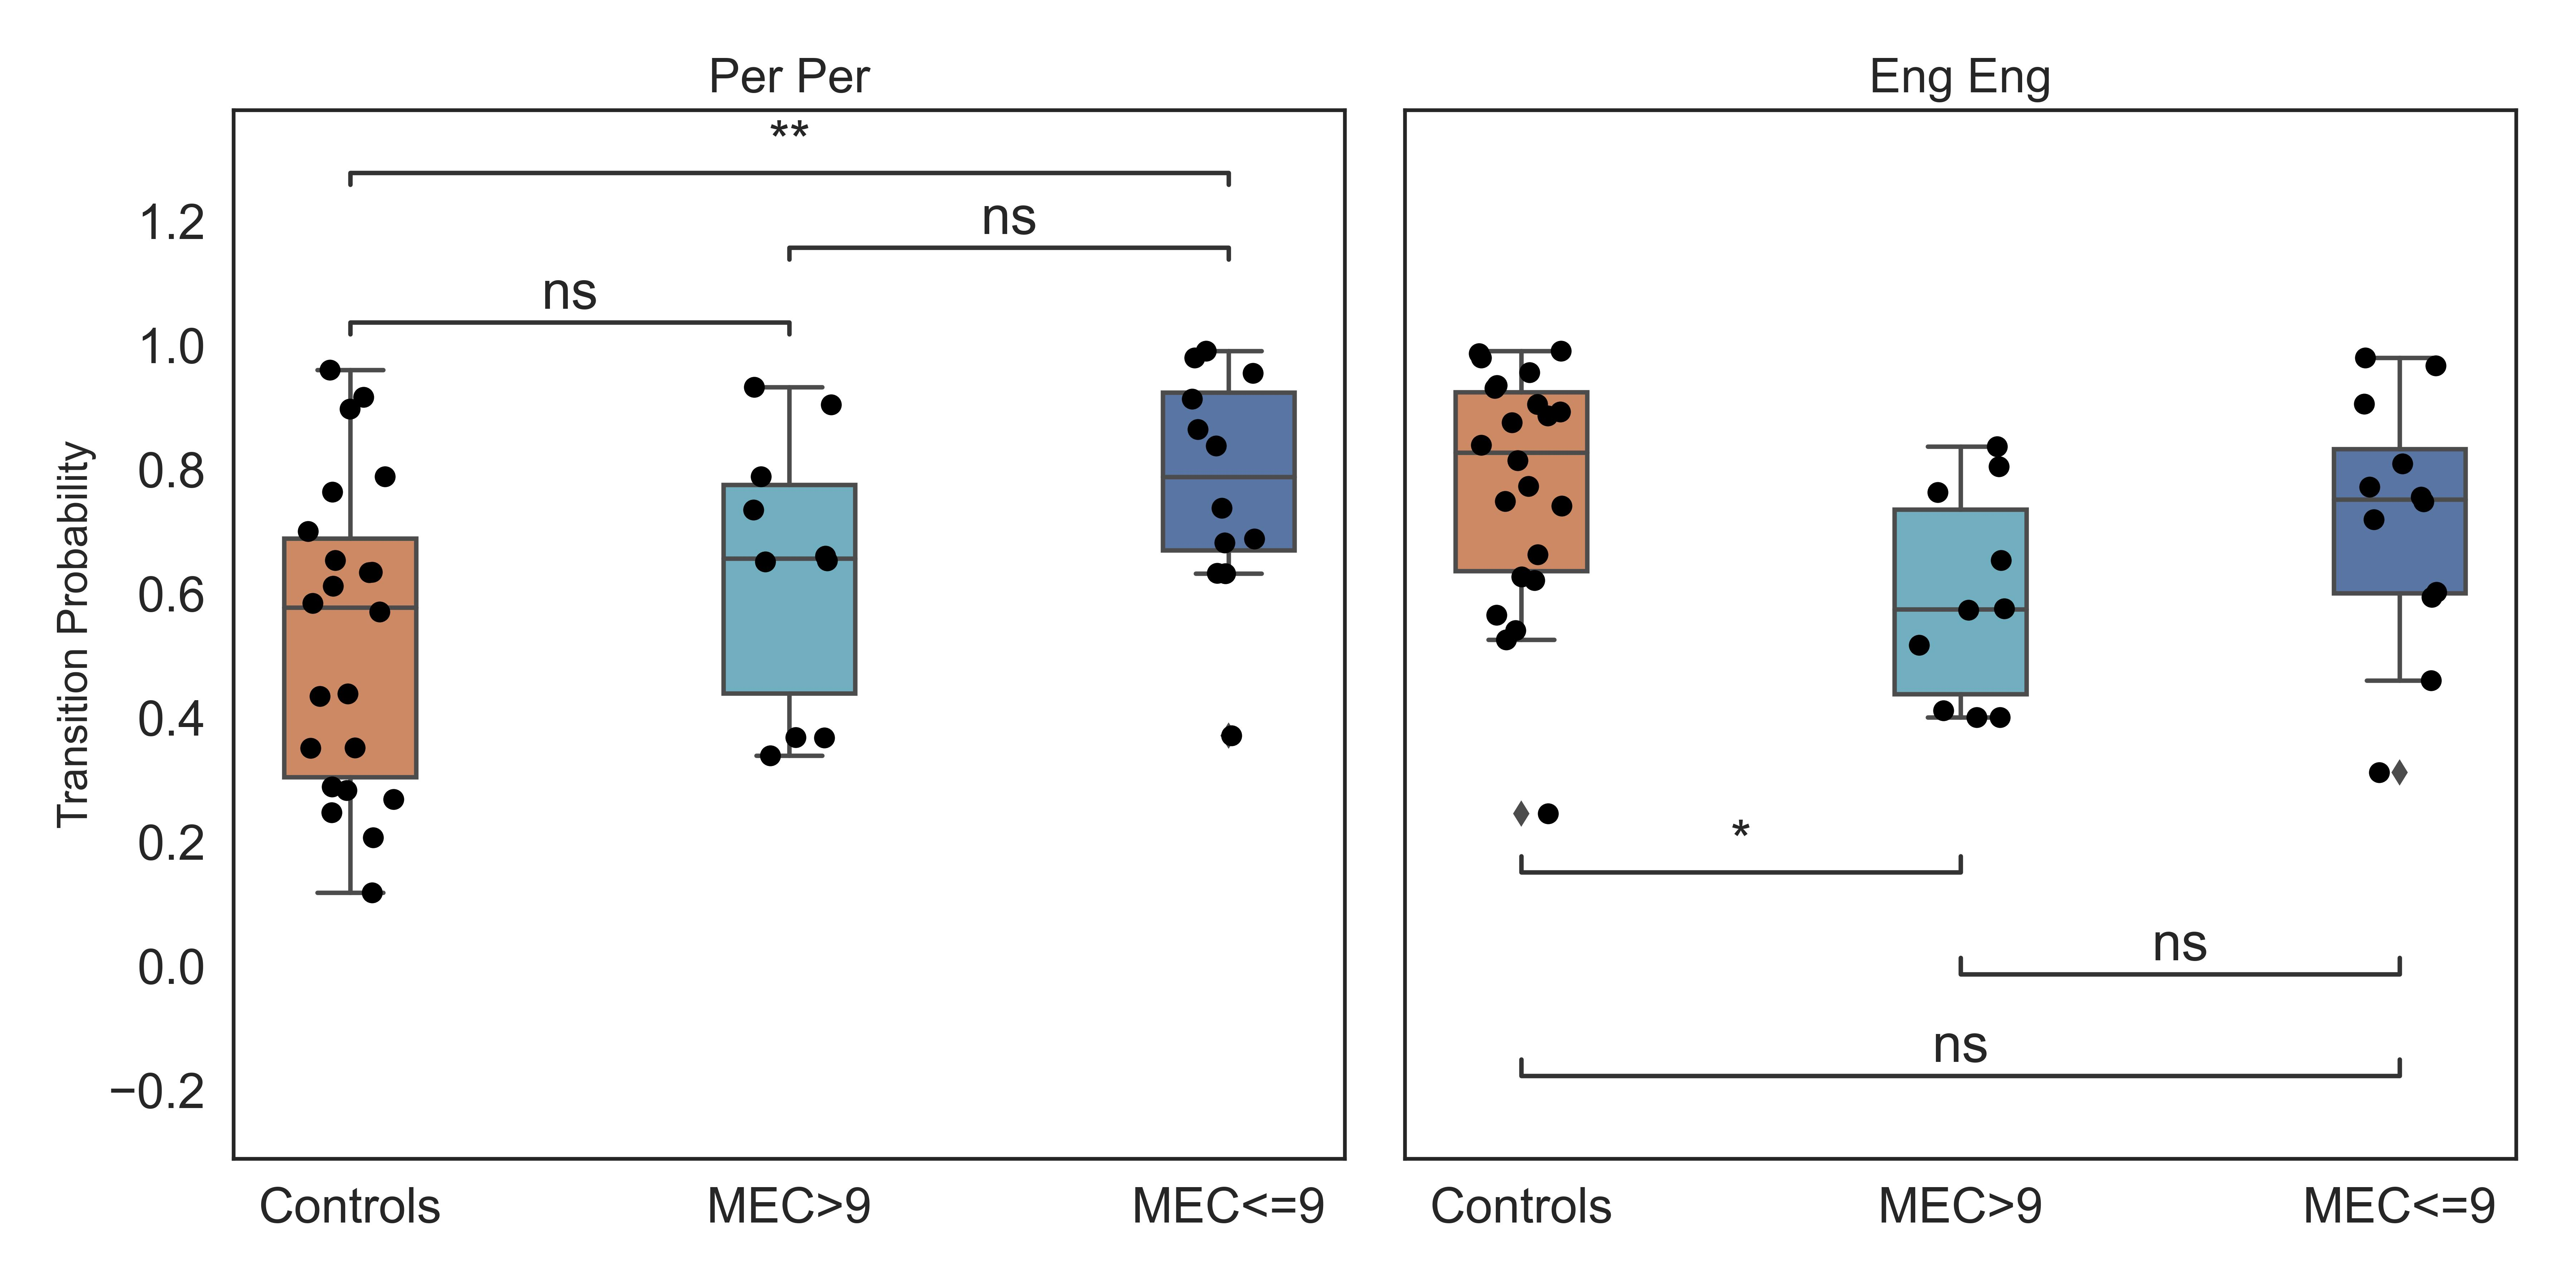
\includegraphics[width=17cm,height=7cm]{MainLayout/Images/chapter8/sticky_state.jpg}
    \caption{Main Title for First Image \\ \small Subtitle for the first graphic.}
    \label{fig:sticky_state}
\end{figure}
We investigated whether the newly identified biomarkers transition probabilities are related to old biomarkers kernel similarity and internal noise by performing a regression analysis on data from both patients and controls. The goal was to determine whether transition probabilities could predict kernel similarity and internal noise levels. Our results indicate that the probability of transitioning to the engaged state is significantly associated with kernel similarity across all three kernel estimation methods (CI, GLM, and HMM), as well as with internal noise estimated by GLM. However, no significant relationships were found between transition probability to the perseverative state and kernel similarity or internal noise. This aligns with our previous findings, where the probability of entering perseveration did not significantly differ between patients and controls, suggesting that the key distinguishing factor is not how often individuals enter perseveration, but rather how effectively they can transition back to an engaged state.
\begin{figure}[H]
    \centering
    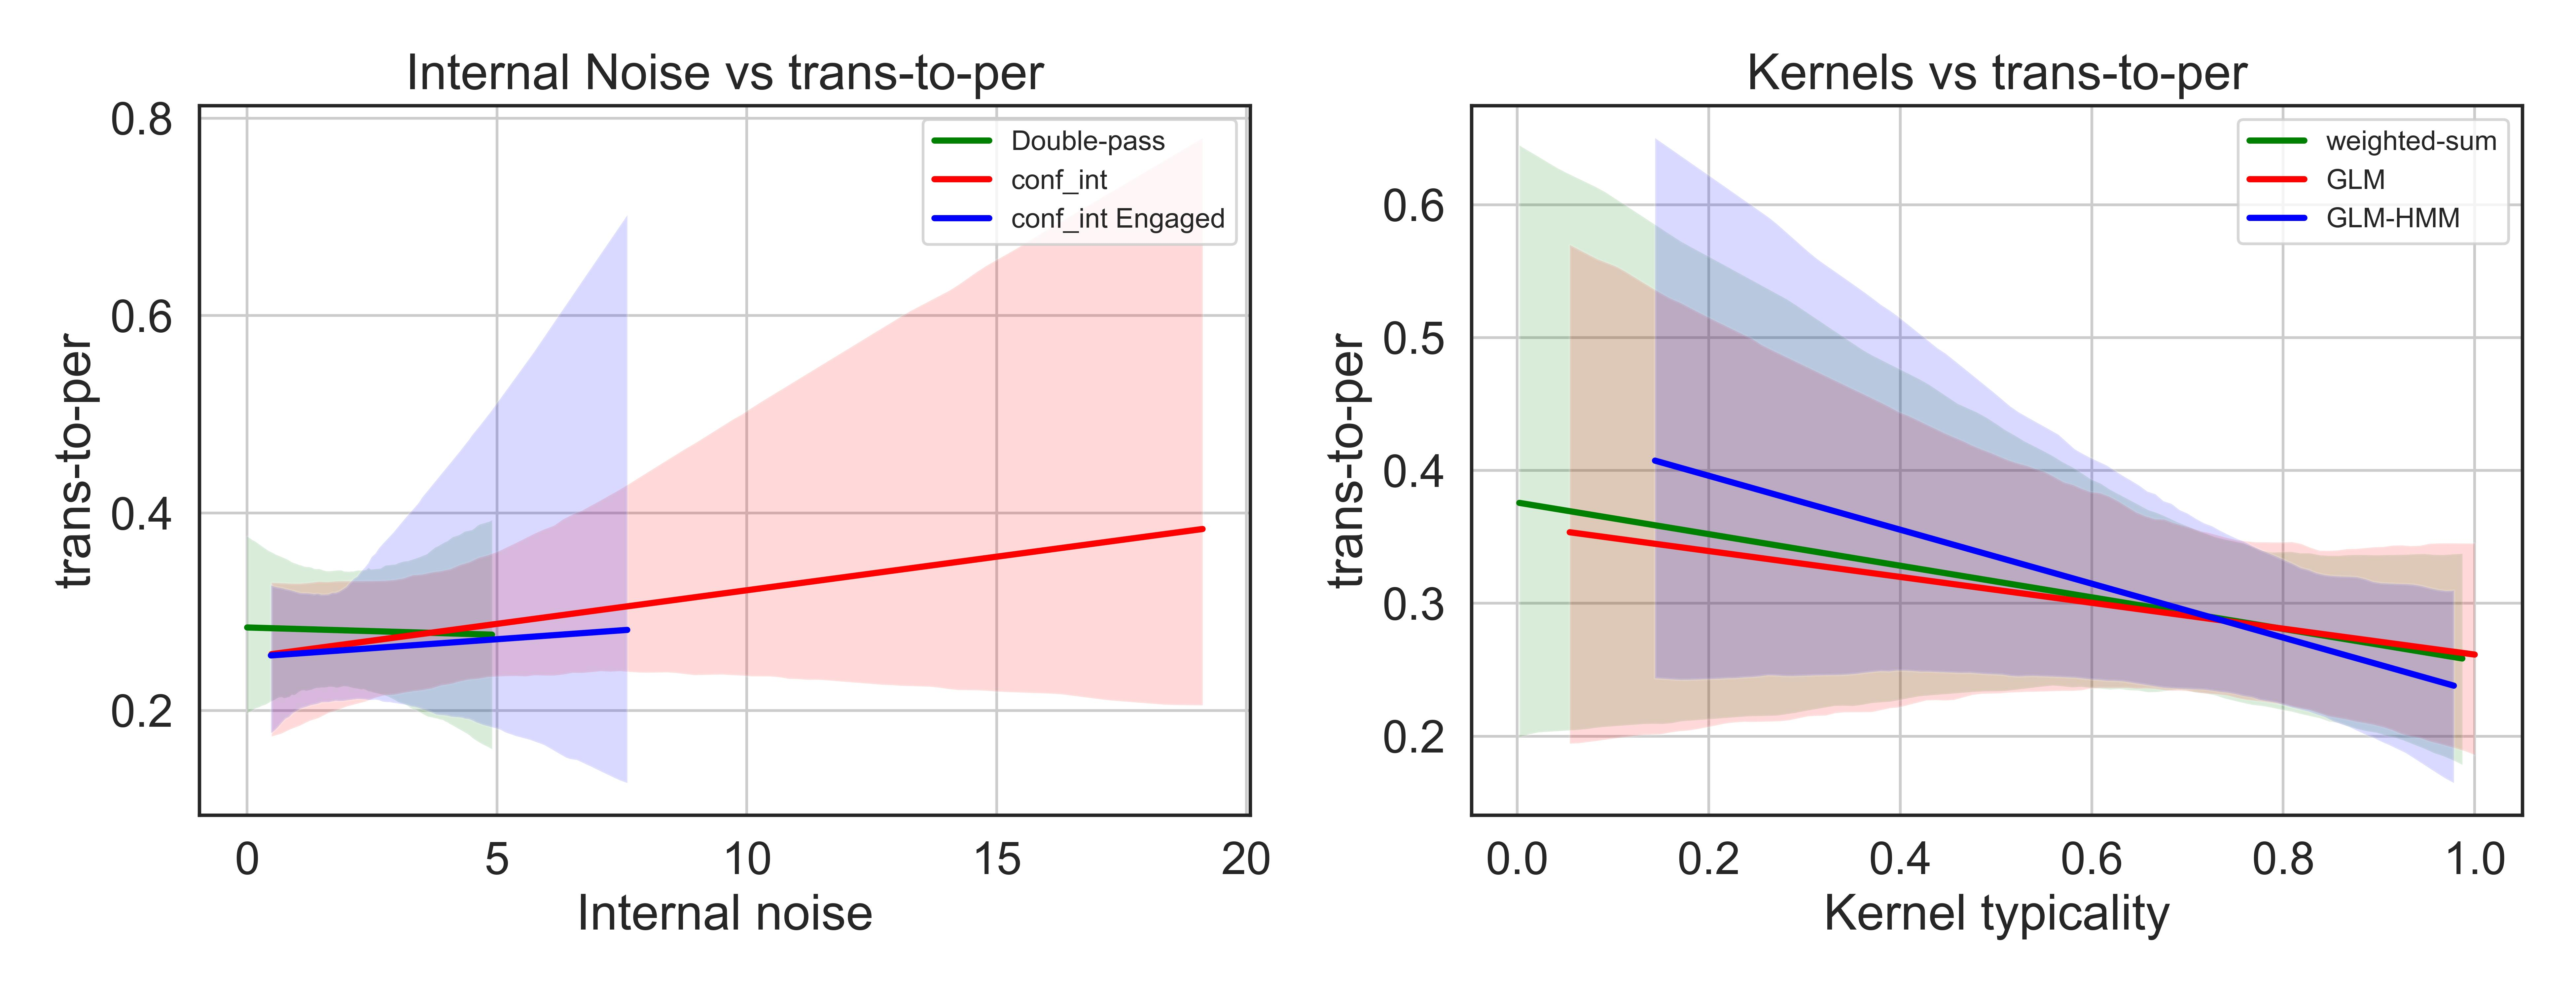
\includegraphics[width=17cm,height=7cm]{MainLayout/Images/chapter8/regression_results_per.jpg}
    \caption{Main Title for First Image \\ \small Subtitle for the first graphic.}
    \label{fig:regression_results_per_per}
\end{figure}
\begin{figure}[H]
    \centering
    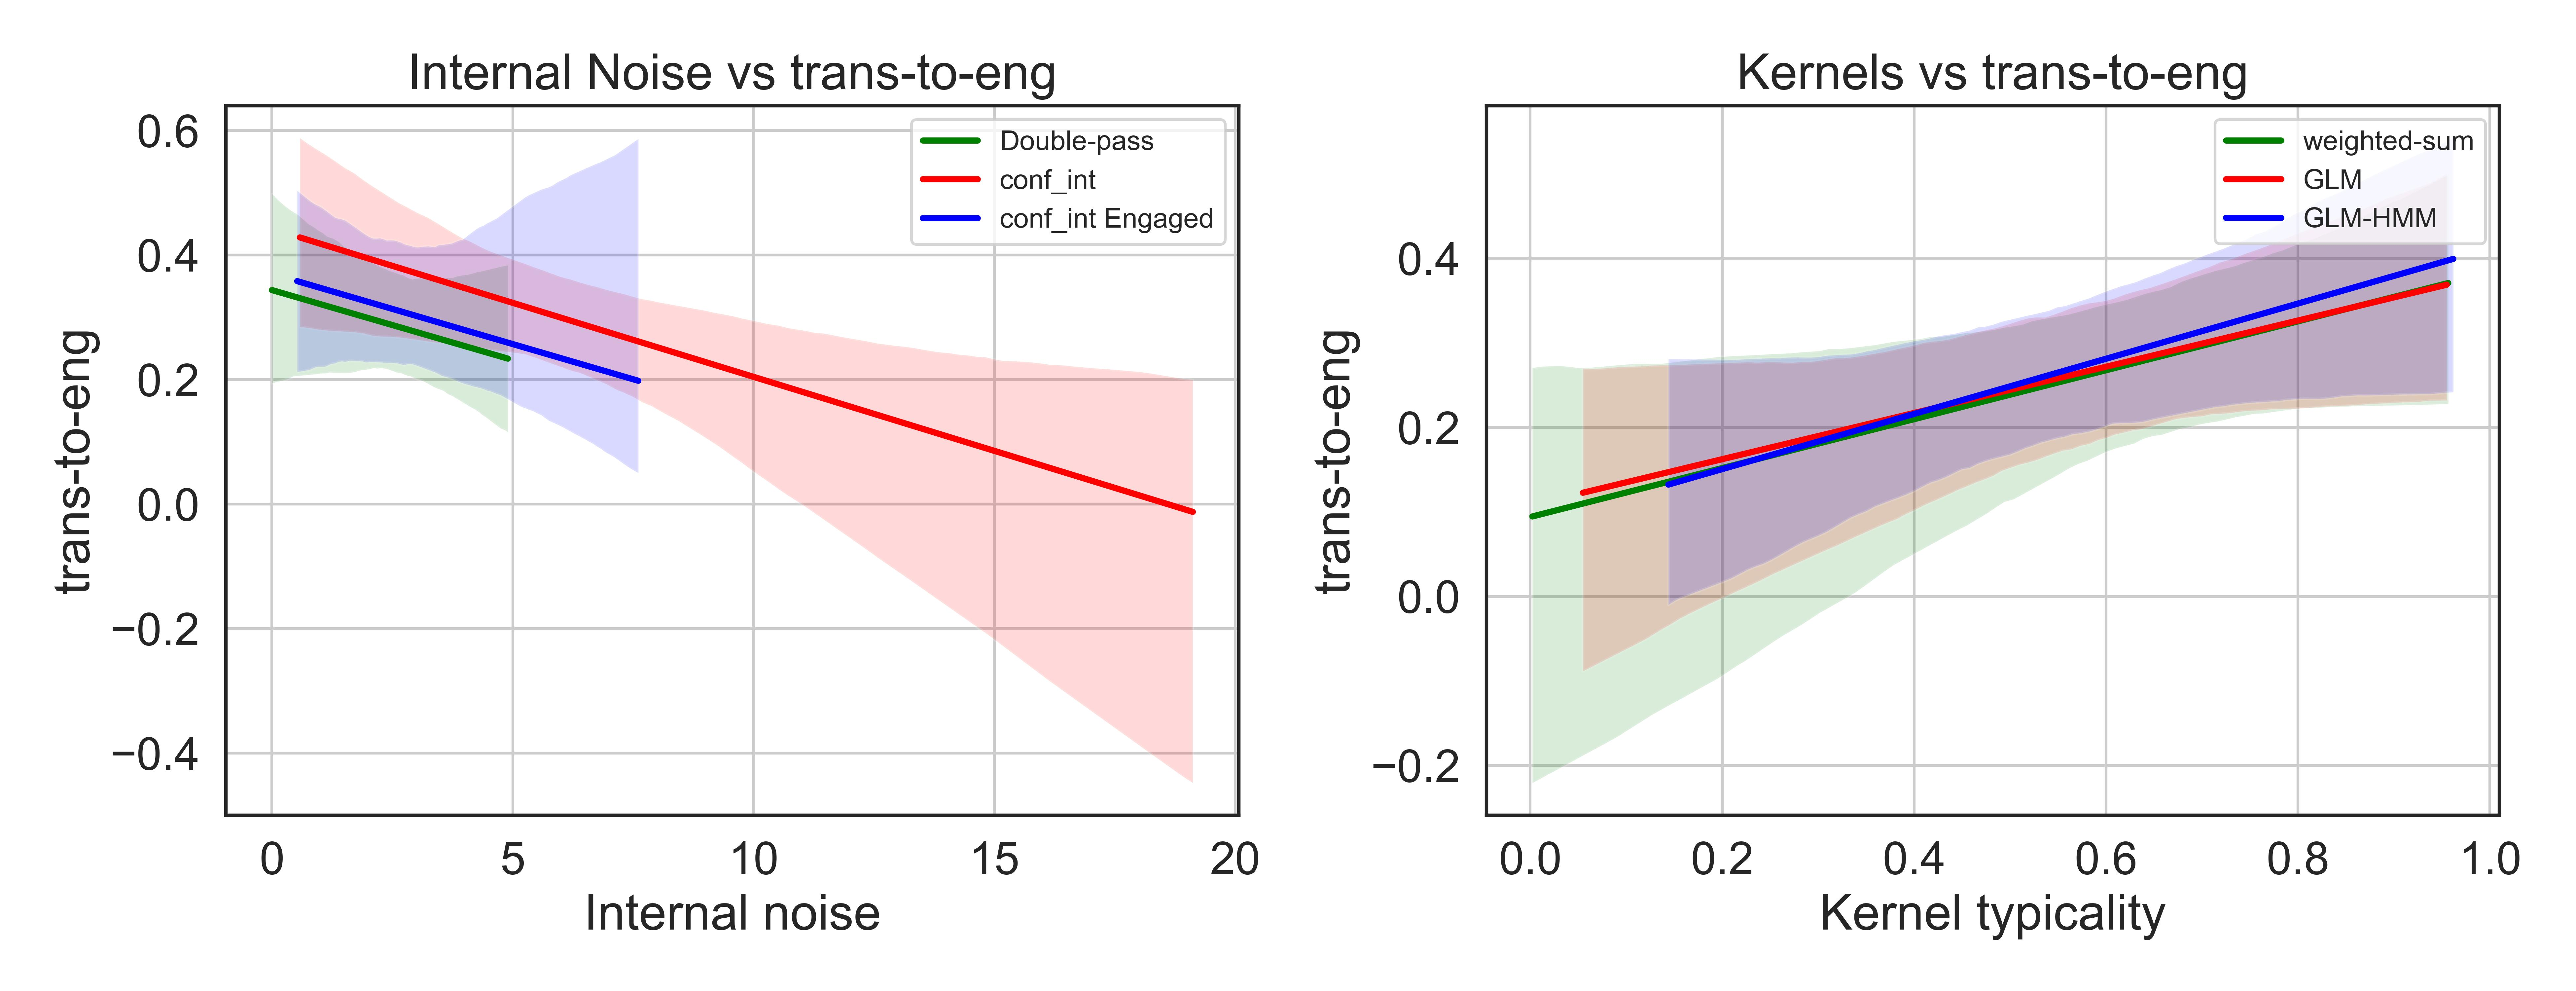
\includegraphics[width=17cm,height=7cm]{MainLayout/Images/chapter8/regression_results_unper.jpg}
    \caption{Main Title for First Image \\ \small Subtitle for the first graphic.}
    \label{fig:regression_results_eng_eng}
\end{figure}
\section{Negative patients differences with controls} 

We compared controls with patients who tested negative for comprehension (MEC-c > 9) and negative for repetition (MEC-r > 9) to examine differences in kernel similarity, internal noise, and transition probabilities.

For patients negative in comprehension (MEC-c > 9), kernel similarity was significantly lower compared to controls across all methods: Kernel CI (p = 0.001, r = -0.67), Kernel GLM (p = 0.001, r = -0.70), and Kernel HMM (p = 0.001, r = -0.73). In terms of internal noise, there was a significant difference in the GLM estimate (p = 0.006, r = 0.58), where patients showed higher internal noise than controls. However, other internal noise estimates (DP, old method, and HMM) showed only marginal trends (p = 0.053 - 0.064), without reaching significance. No significant differences were found in transition probabilities for perseverative or non-perseverative states (p > 0.05), suggesting that state transitions do not strongly differentiate these patients from controls.

For patients negative in repetition (ME-r > 9), kernel similarity was highly significantly lower across all methods: Kernel CI (p = 0.000, r = -0.80), Kernel GLM (p = 0.000, r = -0.83), and Kernel HMM (p = 0.000, r = -0.84), indicating a strong divergence in kernel structure from controls. Internal noise was also significantly higher in this group, with GLM (p = 0.000, r = 0.76), HMM (p = 0.007, r = 0.52), and DP (p = 0.015, r = 0.45) all showing increased noise levels compared to controls. Regarding state transitions, non-perseverative transitions were significantly lower in this group (p = 0.010, r = -0.50), suggesting greater difficulty in returning to an engaged state. However, the difference in perseverative transition probability did not reach significance (p = 0.069).

\section{Quantitative impact on old analysis}

\subsection {Correlation with MEC} 
We analyzed the relationship between GLM-HMM-derived measures and MEC scores to determine whether kernel similarity, internal noise, or transition probabilities were predictive of communication abilities. The regression results (Figure \ref{fig:regression_results_mec}) indicate no significant correlation between MEC scores and kernel similarity (CI, GLM, or HMM), internal noise, or transition probabilities (p > 0.05), suggesting that these metrics do not strongly predict the MEC performance.  
For kernel similarity, the relationships were positive but non-significant, meaning that higher kernel similarity does not systematically relate to better MEC scores (Kernel CI: $\beta$ = 2.93, p = 0.40; Kernel GLM: $\beta$ = 3.34, p = 0.33; Kernel HMM: $\beta$ = -1.77, p = 0.61). For internal noise, the relationships were negative, indicating that higher internal noise may be associated with lower MEC scores, though not significantly (Old method: $\beta$ = -0.80, p = 0.07; GLM: $\beta$ = -0.26, p = 0.16; HMM: $\beta$ = -0.23, p = 0.60). Notably, the old internal noise measure was nearly significant but is no longer after removing perseverative trials in HMM, suggesting that previously observed effects may have been inflated by perseveration rather than reflecting true perceptual variability.

For transition probabilities, higher transition to the engaged state ($\beta$ = 5.97, p = 0.18) was positively associated with MEC scores, suggesting that more frequent return to an engaged state may weakly relate to better communication ability, though not significantly. Transition to perseveration was also positively associated ($\beta$ = 1.04, p = 0.81), implying that perseverative tendencies do not strongly differentiate MEC performance.
\begin{figure}[H]
    \centering
    
\includegraphics[width=17cm,height=7cm]{MainLayout/Images/chapter8/regression_results_mec.jpg}
    \caption{Main Title for First Image \\ \small Subtitle for the first graphic.}
    \label{fig:regression_results_mec}
\end{figure}
When focusing on prosody comprehension (MEC-C, Figure \ref{fig:regression_results_mec_c}), we found a significant negative correlation between MEC-C and internal noise from the old method ($\beta$ = -0.62, p = 0.043), suggesting that patients with higher internal noise in double-pass trials may struggle more with prosody comprehension. However, internal noise from HMM was not significantly correlated, implying that this association in the old method might be driven by perseveration rather than true perceptual variability. Kernel similarity (Kernel CI: $\beta$ = 3.25, p = 0.18; Kernel GLM: $\beta$ = 3.29, p = 0.16; Kernel HMM: $\beta$ = -0.19, p = 0.94) and transition probabilities (Perseverative: $\beta$ = 3.83, p = 0.22; Engaged: $\beta$ = 3.27, p = 0.27) showed no significant relationships with prosody comprehension.
\begin{figure}[H]
    \centering
    
\includegraphics[width=17cm,height=7cm]{MainLayout/Images/chapter8/regression_results_mec_c.jpg}
    \caption{Main Title for First Image \\ \small Subtitle for the first graphic.}
    \label{fig:regression_results_mec_c}
\end{figure}
For prosody repetition (MEC-R, Figure \ref{fig:regression_results_mec_r}), none of the predictors showed a significant relationship with kernel similarity, internal noise, or state transitions (p > 0.05), indicating that repetition performance is not strongly associated with these computational measures. Notably, the old method previously showed a weak negative correlation ($\beta$ = -0.18, p = 0.37), but this relationship is no longer present in HMM ($\beta$ = 0.02, p = 0.93), further suggesting that the previous measure captured perseveration effects rather than genuine perceptual noise.           
\begin{figure}[H]
    \centering
    
\includegraphics[width=17cm,height=7cm]{MainLayout/Images/chapter8/regression_results_mec_r.jpg}
    \caption{Main Title for First Image \\ \small Subtitle for the first graphic.}
    \label{fig:regression_results_mec_r}
\end{figure}

\subsection {Correlation with Airtac} 
Regression analysis with AIRTAC (auditory processing ability) revealed strong significant relationships between kernel similarity and AIRTAC scores (p < 0.01, Figure \ref{fig:regression_results_airtac}), indicating that higher kernel similarity is associated with better auditory discrimination (Kernel CI: $\beta$ = 12.08, p = 0.009; Kernel GLM: $\beta$ = 11.28, p = 0.007; Kernel HMM: $\beta$ = 12.72, p = 0.003).

For internal noise, the old method was significantly negatively correlated with AIRTAC ($\beta$ = -1.20, p = 0.037), meaning that higher noise in double-pass trials was associated with worse auditory discrimination. However, internal noise in HMM ($\beta$ = -0.46, p = 0.49) and GLM ($\beta$ = -0.20, p = 0.36) were not significantly related, suggesting that after removing perseverative trials, internal noise no longer predicts auditory processing abilities.

For transition probabilities, higher transition to the engaged state ($\beta$ = 5.17, p = 0.51) was positively associated with AIRTAC, suggesting that patients who return to engagement more frequently tend to perform better in auditory processing, though not significantly. Conversely, transition to perseveration ($\beta$ = 0.31, p = 0.95) was slightly positively associated with AIRTAC but not meaningful
\begin{figure}[H]
    \centering
    
\includegraphics[width=17cm,height=7cm]{MainLayout/Images/chapter8/regression_results_airtac.jpg}
    \caption{Main Title for First Image \\ \small Subtitle for the first graphic.}
    \label{fig:regression_results_airtac}
\end{figure}
For AIRTAC duration discrimination (Figure \ref{fig:regression_results_airtac_dur_discr}), kernel similarity across all three methods was significantly correlated with better discrimination (p < 0.05). Additionally, the old internal noise measure was negatively correlated ($\beta$ = -0.82, p = 0.007), but this effect disappears in HMM ($\beta$ = -0.27, p = 0.45), again suggesting that the previous effect may have been driven by perseveration.
\begin{figure}[H]
    \centering
    
\includegraphics[width=17cm,height=7cm]{MainLayout/Images/chapter8/regression_results_airtac_dur_discr.jpg}
    \caption{Main Title for First Image \\ \small Subtitle for the first graphic.}
    \label{fig:regression_results_airtac_dur_discr}
\end{figure}
For AIRTAC intensity discrimination (Figure \ref{fig:regression_results_airtac_int_discr}), only kernel similarity showed significant correlations (p < 0.05), while internal noise estimates were not predictive. Transition probabilities were not significantly related, but transition to the engaged state ($\beta$ = 3.89, p = 0.39) had a weak positive association, suggesting that patients who return to engagement more often may have slightly better intensity discrimination.
\begin{figure}[H]
    \centering
    
\includegraphics[width=17cm,height=7cm]{MainLayout/Images/chapter8/regression_results_airtac_int_discr.jpg}
    \caption{Main Title for First Image \\ \small Subtitle for the first graphic.}
    \label{fig:regression_results_airtac_int_discr}
\end{figure}
\subsection {Correlation with other clinical measures} 
LAMA precision measures auditory attentional control, reflecting a participant’s ability to stay engaged in a stimulus-driven task. The regression results (Figure \ref{fig:regression_results_lama_prec}) show that internal noise from HMM was significantly negatively correlated with LAMA precision ($\beta$ = -0.21, p = 0.0004), this suggests that after removing perseverative trials, patients can better perform stimulus-driven tasks, highlighting a link between attentional control and reduced internal noise in engaged trials.

Interestingly, the old internal noise measure was negatively correlated but not significant ($\beta$ = -0.10, p = 0.24), suggesting that the previously observed effect was amplified by perseveration. Transition probabilities were not significantly related, but transition to the engaged state ($\beta$ = 0.34, p = 0.72) showed a weak positive association. This suggests that after removing perseverative trials, patients can better perform stimulus-driven tasks, highlighting a link between attentional control and reduced internal noise in engaged trials.
\begin{figure}[H]
    \centering
    
\includegraphics[width=17cm,height=7cm]{MainLayout/Images/chapter8/regression_results_lama_prec.jpg}
    \caption{Main Title for First Image \\ \small Subtitle for the first graphic.}
    \label{fig:regression_results_lama_prec}
\end{figure}
For MBEA total scores (Figure \ref{fig:regression_results_mbea_total}), no significant relationships were found with any predictors (p > 0.05). However, the old internal noise measure had a weak positive relationship ($\beta$ = 0.05, p = 0.97), which shifted to a negative trend in HMM ($\beta$ = -1.51, p = 0.45), suggesting that perseveration may have contributed to false positive noise effects in prior estimates.

\begin{figure}[H]
    \centering
    
\includegraphics[width=17cm,height=7cm]{MainLayout/Images/chapter8/regression_results_mbea_total.jpg}
    \caption{Main Title for First Image \\ \small Subtitle for the first graphic.}
    \label{fig:regression_results_mbea_total}
\end{figure}
For HADS (anxiety and depression scale, Figure \ref{fig:regression_results_hads}), significant correlations were found with internal noise from HMM ($\beta$ = 2.28,p = 0.003), GLM ($\beta$ = 0.95,p = 0.016), and the old method ($\beta$ = 2.30, p = 0.018), as well as with kernel similarity estimated using HMM ($\beta$=-16.31p = 0.029). This suggests that higher internal noise is associated with increased psychological distress, indicating that patients with more perceptual instability may experience greater emotional difficulties. Additionally, the significant correlation with kernel similarity from HMM suggests that after removing perseverative trials, patients with higher anxiety or depression symptoms may still exhibit altered stimulus-driven processing. 
For transition probabilities, neither transition to perseveration ($\beta$ = -0.62, p = 0.95) nor transition to the engaged state ($\beta$ = -12.80, p = 0.17) were significantly related.
\begin{figure}[H]
    \centering
    
\includegraphics[width=17cm,height=7cm]{MainLayout/Images/chapter8/regression_results_hads.jpg}
    \caption{Main Title for First Image \\ \small Subtitle for the first graphic.}
    \label{fig:regression_results_hads}
\end{figure}
\section{Discussion of the differences} 
The comparison of different methods for measuring internal representation—weighted sum (Classification Image), GLM, and GLM-HMM (GLM in the engaged state)—revealed no significant differences between the controls and patient groups. This suggests that the way internal representations are extracted does not strongly differentiate patients based on prosody comprehension or repetition deficits.

However, the methods used to estimate internal noise showed clear differences. In the old method (double-pass trials), internal noise was artificially limited to 5 standard deviations, whereas in GLM-based estimation, no such constraints were applied, leading to naturally higher noise estimates across all trials. The key finding was that after removing perseverative trials in GLM-HMM, internal noise decreased significantly in both patient groups, showing that a large portion of the high noise estimates in GLM were likely inflated by perseverative responses rather than true perceptual variability. Notably, the internal noise estimated from GLM-HMM was even lower than that from the GLM noise and as well old double-pass measure, suggesting that perseveration had a strong impact on previous noise estimates and that removing these trials provides a more precise measure of true internal noise.

Regarding state transitions, we did not observe a significant difference between controls and patients in their probability of transitioning into the perseverative state. This indicates that perseveration is not exclusive to patients—controls can also exhibit repetitive, non-stimulus-driven responses. However, the critical distinction was in the ability to exit the perseverative state and return to the engaged state. Patients showed a greater tendency to remain stuck in perseveration, struggling to return to an engaged, stimulus-driven behavior, whereas controls were able to transition back more easily, maintaining a flexible and adaptive response pattern.

These findings suggest that the primary deficit in patients is not an increased tendency to enter perseveration but rather an impaired ability to recover from it. This inability to return to an engaged state may be a key factor in the observed difficulties in stimulus-driven perception and auditory attention, reinforcing the importance of distinguishing engaged trials from perseverative ones when assessing perceptual and cognitive flexibility.
\begin{figure}[H]
    \centering
    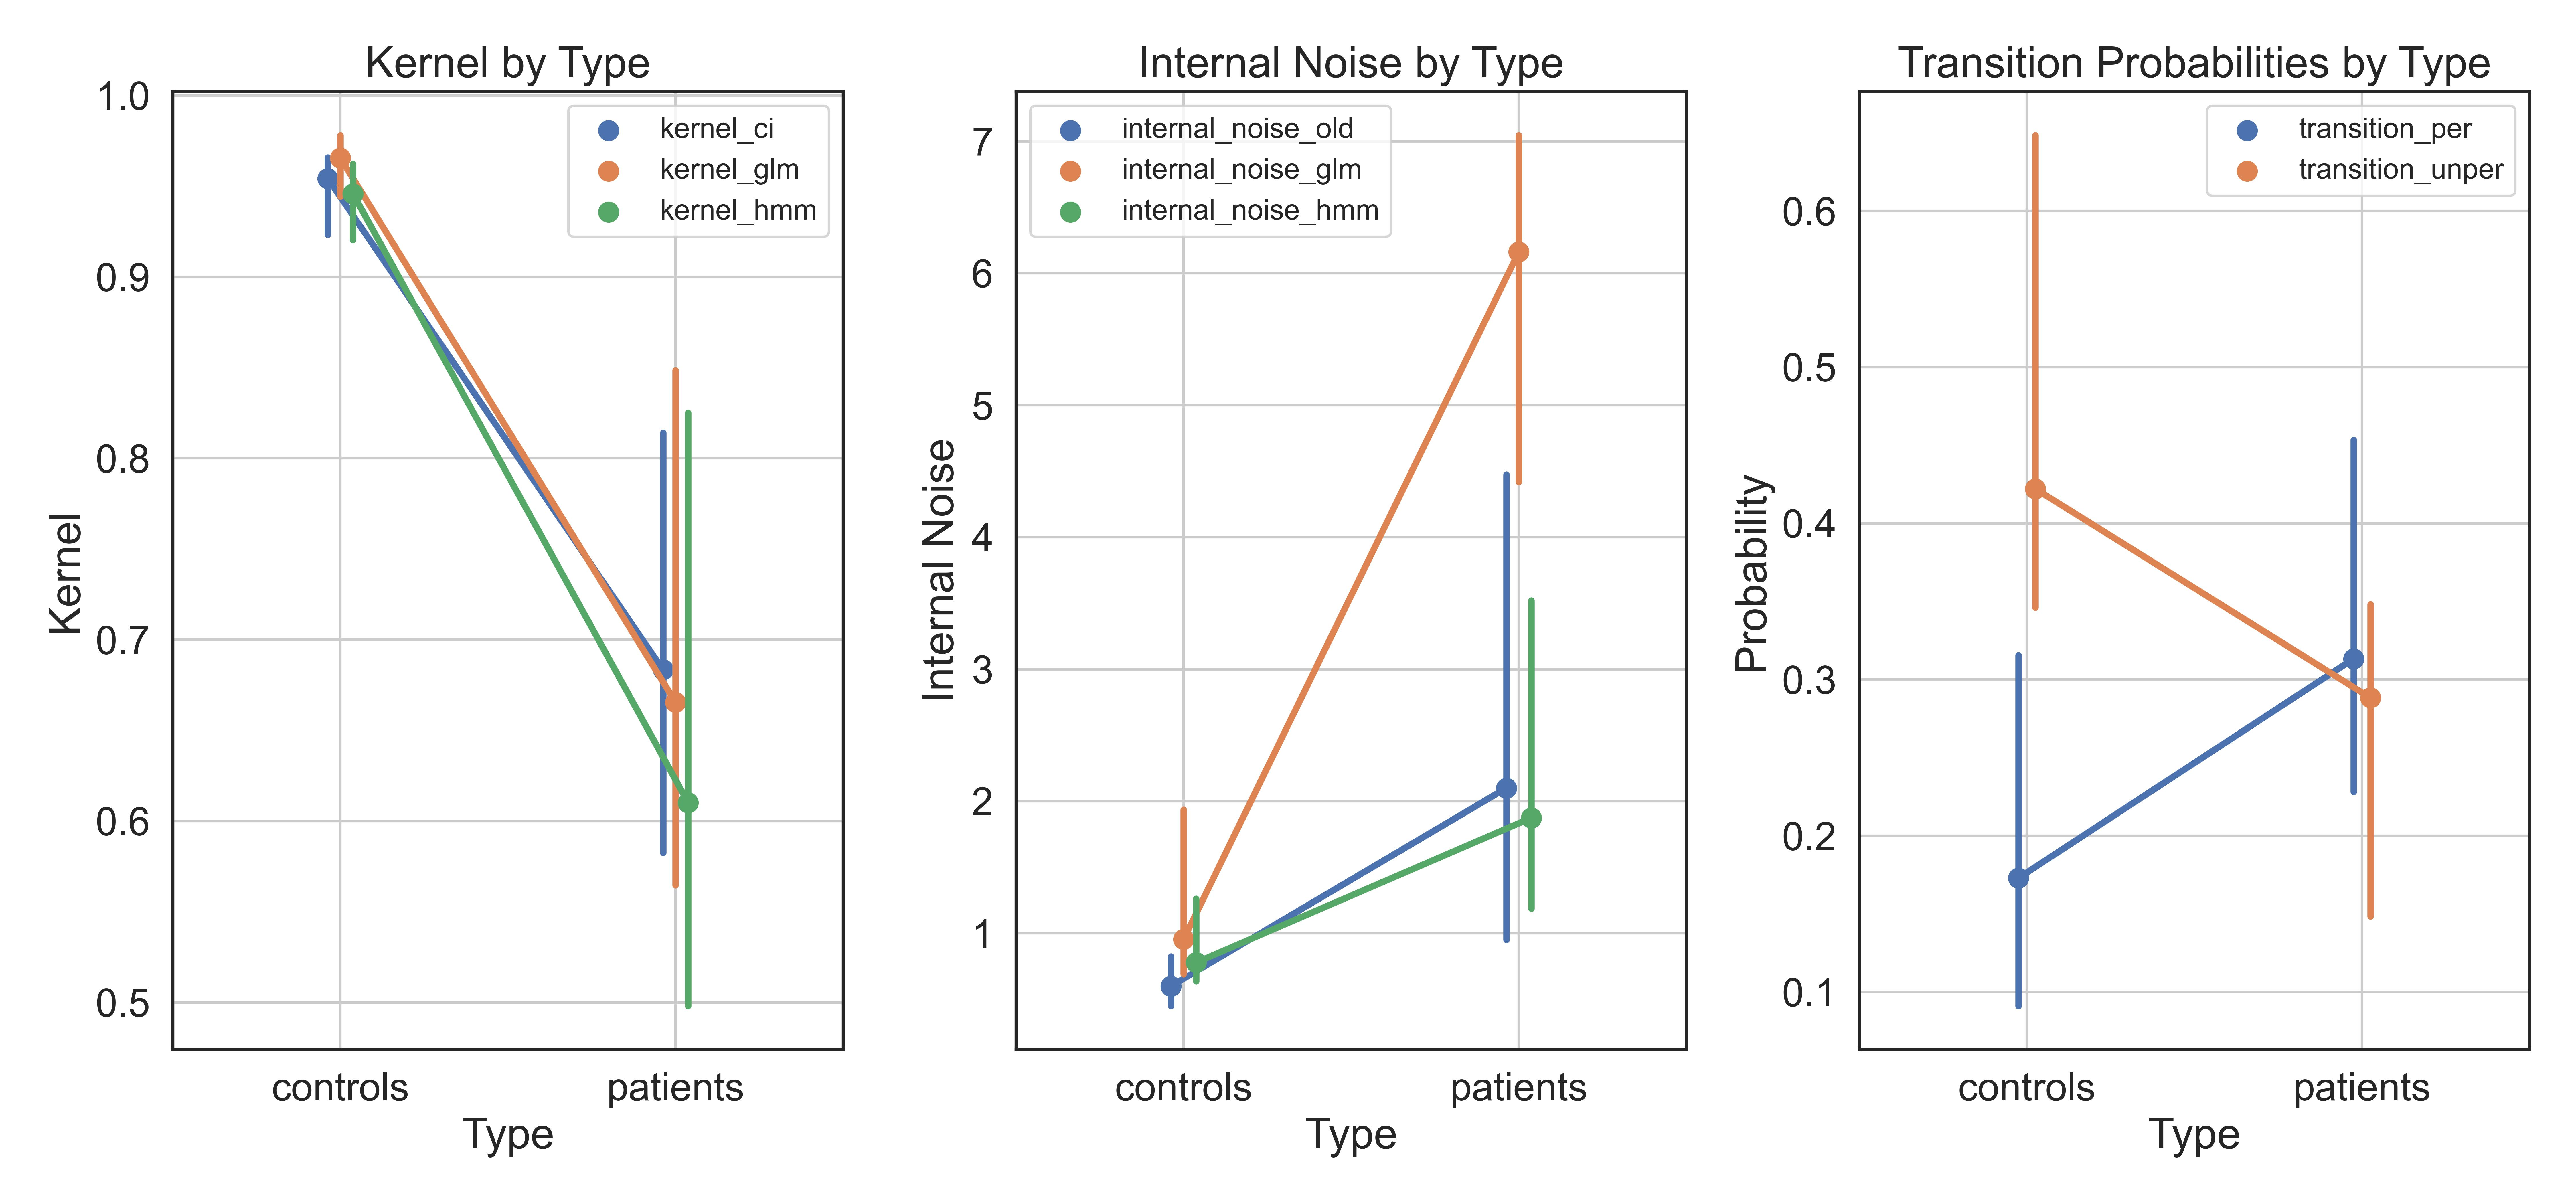
\includegraphics[width=17cm,height=7cm]{MainLayout/Images/chapter8/revcor_measures.jpg}
    \caption{Main Title for First Image \\ \small Subtitle for the first graphic.}
    \label{fig:revcor_measures}
\end{figure}
